\documentclass{beamer}
\usetheme{Madrid}
\usepackage[italian]{babel}
\usepackage[latin1]{inputenc}
\usepackage[T1]{fontenc}
\usepackage{amsmath,amsfonts,amssymb,amsthm}
\usepackage{tikz-network}
\usepackage{graphics}
\usepackage{pgfplots}
 \pgfplotsset{compat=newest}
  \usetikzlibrary{plotmarks}
  \usetikzlibrary{arrows.meta}
  \usepgfplotslibrary{patchplots}
  \usepackage{grffile}
\usepackage{tikz}
\pgfplotsset{plot coordinates/math parser=false}
  \newlength\figureheight
 \newlength\figurewidth

\newcommand{\spa}{\mathbin{\textcolor{white}{-}}} 
\newcommand{\angol}[1]{\langle #1 \rangle}
\newcommand{\tonde}[1]{\left( #1 \right)}
\theoremstyle{definition}
\newtheorem{defn}{Definizione}
\theoremstyle{plain}
\newtheorem{thm}{Teorema}

\title[]{Il Modello Epidemiologico SIR \\ sulle Reti Complesse}
\author{Simmaco Di Lillo }
\date{\today}
\institute{Universit\`a di Pisa}
\logo{
\includegraphics[width=15mm]{Figure/stemma_unipi.png}}

\begin{document}
\begin{frame}
\titlepage
\end{frame}
\begin{frame}
\frametitle{Il modello SIR scalare}
    Il modello SIR \`e un modello compartimentale: la popolazione viene suddivisa in $3$ classi 
    \begin{itemize}
    \item $S$: i suscettibili;
    \item $I$: gli infetti;
    \item $R$: i rimossi.
    \end{itemize}
\end{frame}
\begin{frame}{Il modello SIR scalare}
\begin{figure}
\centering
\begin{tikzpicture}
  \Vertex[x=0,shape = rectangle,label=S,size=1]{S}
  \Vertex[x=3,shape = rectangle,label=I,size=1]{I}
  \Vertex[x=6,shape = rectangle,label=R,size=1]{R}
  \Edge[Direct,label=$\beta I$](S)(I)   \Edge[Direct,label = $\alpha$](I)(R)
  \end{tikzpicture}
  \caption{Schema del modello SIR.}
  \pause
  \begin{equation}
  \begin{aligned}
      \dot{S} =& -\beta S I \\
      \dot{I} = & \spa \beta S I - \alpha I  \\
      \dot{R} = & \spa \alpha I 
      \end{aligned}
  \end{equation}
  \end{figure}
    
\end{frame}
\begin{frame}
\frametitle{Il modello SIR bottom-up su una rete}
\framesubtitle{Un primo esempio}
\begin{figure}
\centering
\begin{tikzpicture}
  \Vertex[x=0,label=$1$,size=1]{S}
  \Vertex[x=3,label=$2$,size=1]{I}
  \Vertex[x=6,label=$3$,size=1]{R}
  \Edge(S)(I)   \Edge(I)(R)
  \end{tikzpicture}
  \end{figure}
  Come si infettano?
  \begin{itemize}
      \item<1-> Il nodo $1$ ha una sola fonte d'infezione.\\
      \only<1>{$\langle S_1\rangle $ diminuisce con un tasso di $\tau \angol{S_1 I_2}$}
      \item<2-> Il nodo $2$ ne ha due.\\
       \only<2>{$\langle S_2\rangle $ diminuisce con un tasso di $\tau \angol{I_1 S_2} +\tau \angol{S_2 I_3}$}
      \item<3-> Anche il  nodo $3$ ne ha una sola.\\
      \only<3>{$\langle S_3\rangle $ diminuisce con un tasso di $\tau \angol{I_2 S_3} $}
  \end{itemize}
\end{frame}
\begin{frame}
    \frametitle{Il modello SIR bottom-up su una rete}
\framesubtitle{Un primo esempio}
\begin{equation*}
\begin{aligned}
	\dot{\angol {S_1}} = & -\tau \angol{ S_1 I_2}, 
\quad &
	\dot{\angol {I_1}} = & \tau \angol{S_1 I_2}-\gamma \angol{I_1}, 
\\
	\dot{\angol {S_2}} = & -\tau \tonde{ \angol{ I_1 S_2} + \angol{S_2I_3}},	
\quad & 
	\dot{\angol {I_2}} = & \tau \tonde{ \angol{ I_1 S_2} + \angol{S_2I_3}}-\gamma \angol{I_2},
\\
	\dot{\angol {S_3}} = & -\tau \angol{ I_2 S_3},
\quad & 
	\dot{\angol {I_3}} = & \tau \angol{ I_2 S_3}-\gamma \angol{I_3},
\end{aligned}
\end{equation*}
\pause
Tale sistema \alert{non \`e chiuso}. Dipende da alcune coppie. 
\end{frame}
\begin{frame}
\frametitle{Il modello SIR bottom-up su una rete}
\framesubtitle{Un primo esempio}
Come evolvono nel tempo le coppie?
    \begin{equation*}
\begin{aligned}
	\dot{\angol{S_1I_2}}=&\spa\tau\angol{S_1S_2I_3} - \tonde{ \tau + \gamma}\angol{S_1 I_2},
\\
	\dot{\angol{I_1S_2}}=&-\tau\angol{I_1S_2I_3} - \tonde{ \tau + \gamma}\angol{I_1 S_2},
\\
	\dot{\angol{S_2I_3}}=&-\tau\angol{I_1S_2I_3} - \tonde{ \tau + \gamma}\angol{S_2 I_3},
\\
	\dot{\angol{I_2S_3}}=&\spa\tau\angol{I_1S_2S_3} - \tonde{ \tau + \gamma}\angol{I_2 S_3}.
	\end{aligned}
\end{equation*}
e le triple?
\begin{equation*}
    \begin{aligned}
        \dot{\angol{S_2I_3}}=&-\tau\angol{I_1S_2I_3} - \tonde{ \tau + \gamma}\angol{I_1 S_2},
\\
	\dot{\angol{S_1S_2I_3}}=&-\tonde{\tau + \gamma}\angol{S_1S_2I_3},
\\
	\dot{\angol{I_1S_2I_3}}=&-\tonde{2\tau + 2\gamma}\angol{I_1S_2I_3},
\\
	\dot{\angol{I_1S_2S_3}}=&-\tonde{\tau + \gamma}\angol{I_1S_2S_3}.
 \end{aligned}
\end{equation*}
\end{frame}
\begin{frame}
      \frametitle{Il modello SIR bottom-up su una rete}
\framesubtitle{Modello generale}
Sia $G = \left( g_{ij}\right)$ la matrice di adiacenza del grafo $G$. L'epidemia si diffonde sul grafo nel seguente modo 
\begin{equation*}
\begin{aligned}
	 \dot{\angol{ S_i}}=& - \sum_{j=1\atop{j\neq i }}^N g_{ij} \angol{ S_i I_j},\\
	 \dot{\angol{I_i}} =&\spa \tau \sum_{j=1\atop{j\neq i}}^N  g_{ij} \angol{ S_i I_j} -\gamma_i \angol{I_i},
\end{aligned}
\end{equation*}
\end{frame}
\begin{frame}
\frametitle{Il modello SIR bottom-up su una rete}
\framesubtitle{Chiusura alle coppie}
Per ottenere un modello chiuso (ma non esatto) possiamo assumere l'indipendenza  a livello delle coppie. Ovvero utilizzare l'approssimazione 
$$ \angol{ A_i B_j } \approx \angol{ A_i }\angol{B_j} \quad \forall A, \, B \in \{ S, \, I,\, R\} \text{ e } \forall (i,j) \in E $$
\pause
\begin{equation*}
 \begin{aligned}
	 \dot{\angol{ S_i}}=& - \sum_{j=1\atop{j\neq i }}^N g_{ij} \angol{ S_i}\angol{ I_j},\\
 	 \dot{\angol{I_i}} =&\spa \tau \sum_{j=1\atop{j\neq i}}^N  g_{ij}  \angol{S_i}\angol{ I_j} -\gamma_i \angol{I_i}.
 \end{aligned}
 \end{equation*}
\end{frame}
\begin{frame}
\frametitle{Il modello SIR bottom-up su una rete}
\framesubtitle{Chiusura alle coppie}
\begin{figure}
    \centering
% This file was created by matlab2tikz.
%
%The latest updates can be retrieved from
%  http://www.mathworks.com/matlabcentral/fileexchange/22022-matlab2tikz-matlab2tikz
%where you can also make suggestions and rate matlab2tikz.
%
\begin{tikzpicture}

\begin{axis}[%
width=6.028in,
height=4.754in,
at={(1.011in,0.642in)},
scale only axis,
xmin=0,
xmax=5,
ymin=0,
ymax=0.35,
axis background/.style={fill=white},
axis x line*=bottom,
axis y line*=left,
legend style={legend cell align=left, align=left, draw=white!15!black}
]
\addplot [color=red, line width=2.0pt]
  table[row sep=crcr]{%
0	0.333333333333333\\
0.000100475457260383	0.333327750896148\\
0.000200950914520766	0.333322167524441\\
0.00030142637178115	0.333316583218443\\
0.000401901829041533	0.333310997978383\\
0.000904279115343449	0.333283057775202\\
0.00140665640164536	0.333255094254932\\
0.00190903368794728	0.333227107446242\\
0.0024114109742492	0.333199097377757\\
0.00492329740575878	0.333058699137463\\
0.00743518383726836	0.332917723672439\\
0.00994707026877794	0.332776174514818\\
0.0124589567002875	0.332634055171426\\
0.0250183888578354	0.331915026764786\\
0.0375778210153833	0.331182255384855\\
0.0501372531729312	0.330436152327952\\
0.0626966853304791	0.329677114738795\\
0.102108236390274	0.327215481818432\\
0.141519787450068	0.324641174996368\\
0.180931338509863	0.321964171028335\\
0.220342889569658	0.31919350535293\\
0.274870838360705	0.315220730809272\\
0.329398787151753	0.311103336256022\\
0.383926735942801	0.306858491220908\\
0.438454684733849	0.302501546535542\\
0.511698843017727	0.296496384111662\\
0.584943001301606	0.290342511122817\\
0.658187159585485	0.284066091588779\\
0.731431317869363	0.277690592664632\\
0.823962581336954	0.269526726473224\\
0.916493844804545	0.261275455659342\\
1.00902510827214	0.252971216615607\\
1.10155637173973	0.244645176809034\\
1.21569652246265	0.23438574594883\\
1.32983667318558	0.224183113794988\\
1.44397682390851	0.214080766948463\\
1.55811697463144	0.204117072879612\\
1.68311697463144	0.193403784285744\\
1.80811697463144	0.182936514271466\\
1.93311697463144	0.172749616737409\\
2.05811697463144	0.162871139436702\\
2.18311697463144	0.153323565735268\\
2.30811697463144	0.144126198180392\\
2.43311697463144	0.135293531088611\\
2.55811697463144	0.126835090981413\\
2.68311697463144	0.118756329228822\\
2.80811697463144	0.11106042130276\\
2.93311697463144	0.10374712141988\\
3.05811697463144	0.0968128382965037\\
3.18311697463144	0.0902514673020522\\
3.30811697463144	0.0840557450763619\\
3.43311697463144	0.0782164406459592\\
3.55811697463144	0.0727224755499841\\
3.68311697463144	0.0675615941436991\\
3.80811697463144	0.0627213396997781\\
3.93311697463144	0.0581884346441867\\
4.05811697463144	0.0539488620496409\\
4.18311697463144	0.0499883521752367\\
4.30811697463144	0.0462930527442834\\
4.43311697463144	0.0428490255007505\\
4.55811697463144	0.0396422733863442\\
4.66858773097358	0.0369947840804212\\
4.77905848731572	0.034512898505142\\
4.88952924365786	0.0321877719670461\\
5	0.0300107450038088\\
};
\addlegendentry{Approssimata}

\addplot [color=blue, line width=2.0pt]
  table[row sep=crcr]{%
0	0.333333333333333\\
0.000100475457260383	0.33332775117652\\
0.000200950914520766	0.333322168645711\\
0.00030142637178115	0.333316585740814\\
0.000401901829041533	0.333311002461736\\
0.000904279115343449	0.333283080450326\\
0.00140665640164536	0.333255149070309\\
0.00190903368794728	0.333227208309998\\
0.0024114109742492	0.333199258157732\\
0.00492329740575878	0.333059366110503\\
0.00743518383726836	0.332919237528702\\
0.00994707026877794	0.332778870981109\\
0.0124589567002875	0.332638265051006\\
0.0250183888578354	0.331931595902953\\
0.0375778210153833	0.331218738109183\\
0.0501372531729312	0.330499530838155\\
0.0626966853304791	0.329773821516115\\
0.0991412937643315	0.327629833725129\\
0.135585902198184	0.32542682709702\\
0.172030510632036	0.323162271980266\\
0.208475119065889	0.320834051099024\\
0.257093885813804	0.317626142783061\\
0.305712652561719	0.314299781871326\\
0.354331419309635	0.310853927218438\\
0.40295018605755	0.307288328954497\\
0.46627950019307	0.302465571513947\\
0.52960881432859	0.297446337787991\\
0.592938128464109	0.292238061528472\\
0.656267442599629	0.286849067385365\\
0.733658471248229	0.280032591279204\\
0.811049499896829	0.272984735524843\\
0.888440528545428	0.265730903942892\\
0.965831557194028	0.258296309197627\\
1.05793596976172	0.249249184589584\\
1.15004038232942	0.240033136540703\\
1.24214479489711	0.230697304828548\\
1.3342492074648	0.221287878081579\\
1.44286725998794	0.210158037529048\\
1.55148531251107	0.199063059012029\\
1.66010336503421	0.188071612582134\\
1.76872141755734	0.177244701902424\\
1.88893196521442	0.165520374303466\\
2.00914251287149	0.154131833198533\\
2.12935306052856	0.143134740860959\\
2.24956360818563	0.132574608346779\\
2.37456360818563	0.12209553959032\\
2.49956360818563	0.112155781376778\\
2.62456360818563	0.102773341814187\\
2.74956360818563	0.0939584472228666\\
2.87456360818563	0.0857132435851595\\
2.99956360818563	0.0780307810161572\\
3.12456360818563	0.0708988244967405\\
3.24956360818563	0.0643015118334588\\
3.37456360818563	0.0582191503589672\\
3.49956360818563	0.0526277151834682\\
3.62456360818563	0.0475016394160471\\
3.74956360818563	0.0428146697023513\\
3.87456360818563	0.0385398175357336\\
3.99956360818563	0.0346492430664406\\
4.12456360818563	0.031115623106694\\
4.24956360818563	0.0279124562820615\\
4.37456360818563	0.0250140892127293\\
4.49956360818563	0.0223957818462954\\
4.62456360818563	0.0200340851137771\\
4.74956360818563	0.0179068527747512\\
4.81217270613922	0.0169229578724849\\
4.87478180409282	0.015990178489161\\
4.93739090204641	0.0151061256192865\\
5	0.0142684938646879\\
};
\addlegendentry{Esatta}

\end{axis}
\end{tikzpicture}%
    \caption{Prevalenza calcolata usando i due modelli. }
 
\end{figure}
    
\end{frame}
{
\logo{}
\begin{frame}
\frametitle{Il modello SIR bottom-up su una rete}
\framesubtitle{Approccio generale alla chiusura}
Diamo due importanti definizioni
    \begin{defn}[cut-vertex]
    Sia $G=(V,E)$ un grafo connesso. $v\in V$ \`e un \textit{cut-vertex} se il grafo senza il nodo $v$ risulta sconnesso.
    \end{defn}
    
    \begin{defn}[Probabilit\`a condizionale]
    Siano $A,B$ due eventi di uno spazio di probabilit\`a con $\mathbb{P}(B)>0$. Si dice \textit{probabilit\`a condizionale} di $A$ dato $B$ la quantit\`a
    $$ \mathbb{P}(A\, \vert B) = \frac{ \mathbb{P}(A\cap B)}{\mathbb{P}(B)}.$$
    \end{defn}
\end{frame}

\begin{frame}
\frametitle{Il modello SIR bottom-up su una rete}
\framesubtitle{Approccio generale alla chiusura}
\begin{thm}
Sia $G=(V,E)$ un grafo e $F=\{ v_1, \dots, v_k\}$ un sottoinsieme connesso di vertici e sia $v_i$ un suo cut-vertex. Poniamo  $$ F_1 = \{ v_1, \dots, v_{i-1}\} \text{ e }  F_2 =\{ v_{i+1}, \dots, v_k\}.$$ 
Se ogni cammino che connette un nodo in $F_1$ ad uno in $F_2$ passa da $v_i$ allora: 
\begin{equation*}\label{cut}\angol{ Z_{v_1}\dots Z_{v_{i-1}} S_{v_i} Z_{v_{i+1}} \dots Z_{v_k}} = \angol{ Z_{v_1}\dots Z_{v_{i-1}} S_{v_i}} \angol{S_{v_i}  Z_{v_{i+1}} \dots Z_{v_k}}	
\end{equation*}
dove $Z\in \{ S,I,R\}$. 
\end{thm}
\end{frame}

\begin{frame}
\frametitle{Il modello SIR bottom-up su una rete}
\framesubtitle{Approccio generale alla chiusura}
\begin{proof}
\only<1>{Se $\angol{S_{v_i}}=0$ allora l'uguaglianza risulta banalmente vera.\\ }
\pause Sia $\angol{S_{v_i}}\neq 0 $
\pause
$$ \angol{ Z_{v_1}\dots Z_{v_{i-1}} S_{v_i} Z_{v_{i+1}}\dots Z_{v_k}} = \angol{ Z_{v_1}\dots Z_{v_{i-1}} S_{v_i} Z_{v_{i+1}}\dots Z_{v_k}\, \vert \, S_{v_i}} \angol{S_{v_i}}.$$
\pause
Notiamo che 
$$ \angol{ Z_{v_1}\dots Z_{v_{i-1}} S_{v_i} Z_{v_{i+1}}\dots Z_{v_k}\, \vert \, S_{v_i}} =$$
$$=\angol{ Z_{v_1}\dots Z_{v_{i-1}} S_{v_i} \, \vert\, S_{v_i}} \angol{S_{v_i}Z_{v_{i+1}}\dots Z_{v_k}\, \vert \, S_{v_i}}.$$ 
Ogni percorso da $F_1$ a $F_2$ deve passare attraverso $v_i$. Poich\`e $v_i$ \`e suscettibile  la trasmissione non pu\`o avvenire tra un nodo in $F_1$ ed uno in $F_2$.\\\pause
Riapplicando la definizione di probabilit\`a condizionale la tesi 
\end{proof}

\end{frame}
}
\begin{frame}
\frametitle{Il modello SIR bottom-up su una rete}
\framesubtitle{Approccio generale alla chiusura}
\begin{itemize}
	\item<1->{Con una visit\`a in profondit\`a si trovano   tutti i cut-vertex di $G$.}
	\item<2->\alt<2>{Si divide la rete originale in sottoreti connesse a due a due scollegate. Le sottoreti vengono create in modo che i cut-vertex siano mantenuti in tutte le sottoreti generate.}{Si divide la rete originale in sottoreti ...}
	\item<3-> \alt<3>{Per ogni nodo $i$ delle sottoreti, si ha}{ Per ogni nodo $i$ delle sottoreti ...}
	\only<3>{
	\begin{equation*}
	\begin{aligned}
\dot{\angol{S_i}} &= -\tau \sum_j g_{ij} \angol{S_iI_j},\\
\dot{\angol{I_i}} &= \tau \sum_j g_{ij} \angol{S_iI_j}-\gamma\angol{I_i},\\
\dot{\angol{R_i}} &= 1 -\angol{S_i} -\angol{I_i}.
		\end{aligned}
	\end{equation*}
	Si possono trovare  equazioni simili anche per le strutture di ordine maggiore (coppie, triple, ...)}
	\item<4-> Nella gerarchia che si verr\`a a creare, se appare un termine composto da  vertici di sottoreti diverse allora in esso \`e presente un cut-vertex suscettibile. Usando il Teorema precedente  \`e possibile esprimere questo termine usando termini pi\`u semplici.
\end{itemize}

\end{frame}
\begin{frame}
\frametitle{Il modello SIR bottom-up su una rete}
\framesubtitle{La rete lollipop}
\begin{columns}
\begin{column}{0.5\textwidth}
   \begin{figure}[!ht]
\centering
\begin{tikzpicture}[scale=0.8]
\Vertex[label=1]{1}
\Vertex[label=2,y=-2]{2}
\Vertex[label=3, y=-1, x=1.73]{3}
\Vertex[label=4, y=-1, x= 3.73]{4}
\Edge(1)(2) \Edge(2)(3) \Edge(1)(3) \Edge(3)(4)
\end{tikzpicture}
\end{figure}
\end{column}
\pause
\begin{column}{0.5\textwidth}  %%<--- here
\begin{figure}[!htb]
\centering
\begin{tikzpicture}[scale=0.8]
\Vertex[label=1]{1}
\Vertex[label=2,y=-2]{2}
\Vertex[label=3, y=-1, x=1.73,color=gray,opacity=0.3]{3}
\Vertex[label=3, y=-1, x= 3.73,color=gray,opacity=0.3]{33}
\Vertex[label=4, y=-1, x=5.73]{4}
\Edge(1)(2) \Edge(2)(3) \Edge(1)(3) \Edge(33)(4)
\end{tikzpicture}
\end{figure}
\end{column}
\end{columns}
\pause
\begin{equation*}
 \begin{aligned}	
 \dot{\angol{S_1I_3}}&=
 \pause  \tau\tonde{ \angol{S_1I_2S_3} 
+ \angol{S_1S_3I_4}} \pause -  \tau  \angol{S_1I_3} \pause - \gamma\angol{S_1 I_3}\pause -\tau \angol{ S_1 I_2 I_3}= \\ \pause
 &= \tau \tonde{ \angol{S_1I_2S_3} + \frac{ \angol{S_1S_3}\angol{S_3 I_4}}{\angol{S_3}}} -\tonde{ \tau + \gamma} \angol{S_1I_3} - \tau \angol{S_1I_2S_3}
 \end{aligned}
 \end{equation*}
\pause
Grazie al Teorema,  il numero di equazioni passa da $35$ a $27$
\end{frame}
\begin{frame}
\frametitle{La rete stradale del Minnesota}
\framesubtitle{Prevalenza e grado }

   \begin{figure}[!ht]
\centering
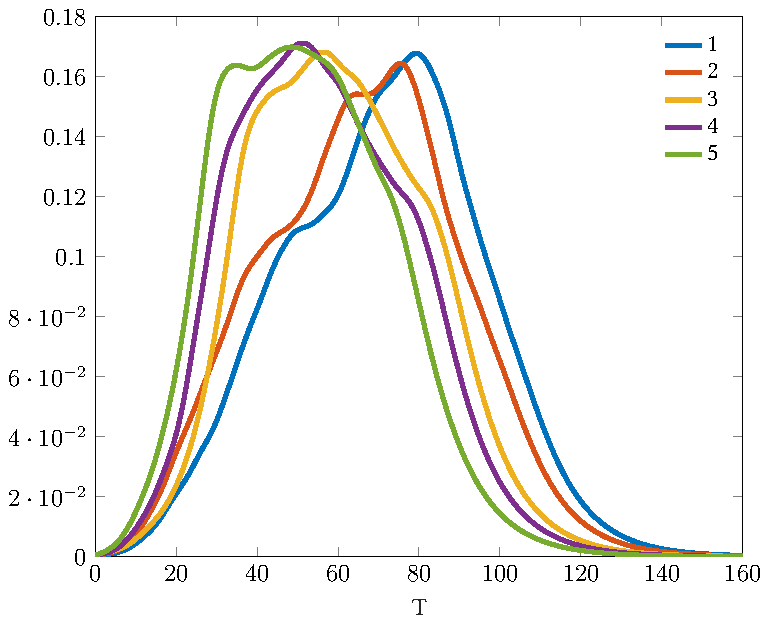
\includegraphics[width=0.5\textwidth]{Figure/minnesota_prevalenza}
\end{figure}
\end{frame}
\begin{frame}
\frametitle{La rete stradale del Minnesota}
\framesubtitle{Immunizzazione}
   \begin{figure}[!ht]
\centering
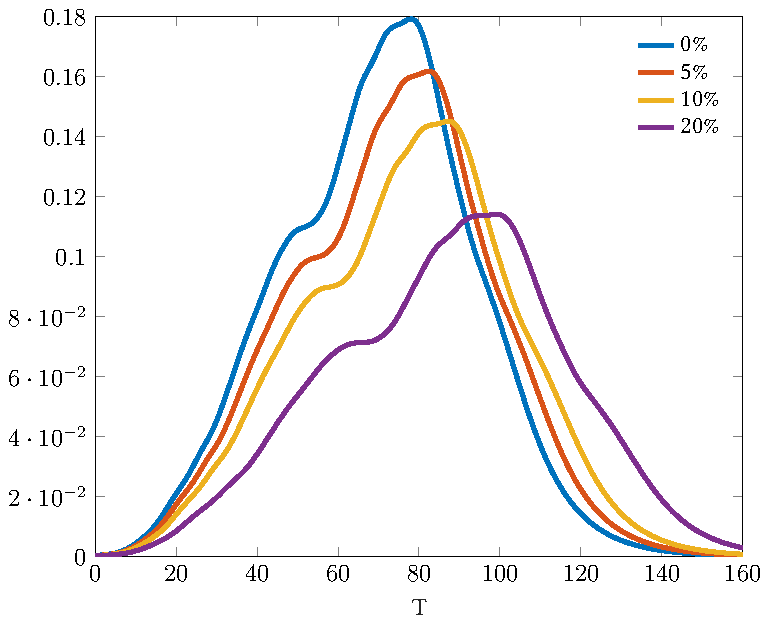
\includegraphics[width=0.5\textwidth]{Figure/minnesota_immunizzazione}
\end{figure}
\end{frame}

\end{document}
